% Three 1-simplices from p to q: the blue and orange are homotopic (rel
% endpoints), but the red one is not, as it goes around the hole.
% Source: book/tex/homology/cohomology.tex (§ Visualization of cohomology groups).
\documentclass[border=2mm]{standalone}
\usepackage{tikz}
\usepackage{amssymb}
\usetikzlibrary{arrows.meta}
\begin{document}
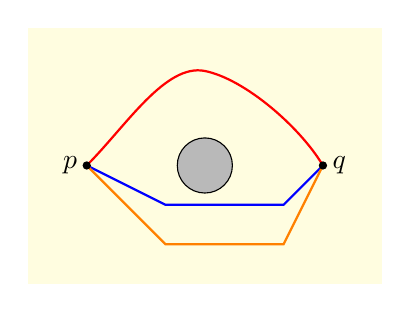
\begin{tikzpicture}[scale=0.5]
  \fill[yellow!12] (-4.5,-3) rectangle (4.5,3.5);
  \fill[gray!55] (0,0) circle (0.7);
  \draw (0,0) circle (0.7);
  \draw[red, thick] (-3,0) .. controls (-2,1) and (-1,2.6) .. (0,2.4) .. controls (1,2.2) and (2.4,1) .. (3,0);
  \draw[blue, thick] (-3,0) -- (-1,-1) -- (2,-1) -- (3,0);
  \draw[orange, thick] (-3,0) -- (-1,-2) -- (2,-2) -- (3,0);
  \fill (-3,0) circle (3pt) node[left] {$p$};
  \fill (3,0) circle (3pt) node[right] {$q$};
\end{tikzpicture}
\end{document}
